\let\negmedspace\undefined
\let\negthickspace\undefined
\documentclass[journal]{IEEEtran}
\usepackage[a5paper, margin=10mm, onecolumn]{geometry}
%\usepackage{lmodern} % Ensure lmodern is loaded for pdflatex
\usepackage{tfrupee} % Include tfrupee package

\setlength{\headheight}{1cm} % Set the height of the header box
\setlength{\headsep}{0mm}     % Set the distance between the header box and the top of the text

\usepackage{gvv-book}
\usepackage{gvv}
\usepackage{cite}
\usepackage{amsmath,amssymb,amsfonts,amsthm}
\usepackage{algorithmic}
\usepackage{graphicx}
\usepackage{textcomp}
\usepackage{xcolor}
\usepackage{txfonts}
\usepackage{listings}
\usepackage{enumitem}
\usepackage{mathtools}
\usepackage{gensymb}
\usepackage{comment}
\usepackage[breaklinks=true]{hyperref}
\usepackage{tkz-euclide} 
\usepackage{listings}
% \usepackage{gvv}                                        
\def\inputGnumericTable{}                                 
\usepackage[latin1]{inputenc}                                
\usepackage{color}                                            
\usepackage{array}                                            
\usepackage{longtable}                                       
\usepackage{calc}                                             
\usepackage{multirow}                                         
\usepackage{hhline}                                           
\usepackage{ifthen}                                           
\usepackage{lscape}
\usepackage{circuitikz}
\tikzstyle{block} = [rectangle, draw, fill=blue!20, 
    text width=4em, text centered, rounded corners, minimum height=3em]
\tikzstyle{sum} = [draw, fill=blue!10, circle, minimum size=1cm, node distance=1.5cm]
\tikzstyle{input} = [coordinate]
\tikzstyle{output} = [coordinate]

\begin{document}


\bibliographystyle{IEEEtran}
\vspace{3cm}

\title{2.9.2}
\author{EE25BTECH11051 - Shreyas Goud Burra}
\maketitle
{\let\newpage\relax\maketitle}

\renewcommand{\thefigure}{\theenumi}
\renewcommand{\thetable}{\theenumi}
\setlength{\intextsep}{10pt}


\numberwithin{equation}{enumi}
\numberwithin{figure}{enumi}
\renewcommand{\thetable}{\theenumi}

\textbf{Question}
If (-5, 3) and (5, 3) are two vertices of an equilateral triangle, then the
coordinates of the third vertex, given that the origin lies inside the triangle (take $\sqrt{3}$ = 1.7), are\\

\solution\\

Let us find the solution theoretically first and then verify it computationally.\\
Let the two given points be represented as vectors, \textbf{A} and \textbf{B}, respectively

\begin{align}
    \textbf{A} = \myvec{-5\\3}, \textbf{B} = \myvec{5\\3}
    \label{0.1}
\end{align}

Let us assume the third point be \textbf{C}.\\
We have to first find the line equation of the line joining the points A and B.

\begin{align}
    \textbf{x} = \textbf{A} + t(\textbf{B}-\textbf{A})
    \label{0.2}
\end{align}

This gives,

\begin{align}
    \textbf{x} = \myvec{-5\\3}+t\myvec{10\\0}
    \label{0.3}
\end{align}

We have to find the lines aligned at $60^{\circ}$ to this line at both \textbf{A} and \textbf{B}.\\
We can get this by multiplying a rotation vector to this vector, this is given by,

\begin{align}
    \textbf{V}(\theta) = \myvec{\cos\theta & -\sin\theta \\\sin\theta & \cos\theta}
    \label{0.4}
\end{align}

By multiplying this to \ref{0.3} with $\theta = \pm 60^{\circ}$, we get the lines,

\begin{align}
    \textbf{x} = \myvec{-5\\3} + t(\textbf{V}(\pm 60^{\circ}))\myvec{1\\0}
    \label{0.5}
\end{align}

The lines we get from this equation are,

\begin{align}
    \textbf{x} = \myvec{-5\\3}+t\myvec{\frac{1}{2}\\\frac{\sqrt{3}}{2}}
    \label{0.6}
\end{align}

\begin{align}
    \textbf{x} = \myvec{-5\\3}+t\myvec{\frac{1}{2}\\\frac{-\sqrt{3}}{2}}
    \label{0.7}
\end{align}

By doing the same thing taking point B,

\begin{align}
    \textbf{x} = \myvec{5\\3}+t\myvec{\frac{1}{2}\\\frac{\sqrt{3}}{2}}
    \label{0.8}
\end{align}

\begin{align}
    \textbf{x} = \myvec{5\\3}+t\myvec{\frac{1}{2}\\\frac{-\sqrt{3}}{2}}
    \label{0.9}
\end{align}

We can get two possible points that fit the given conditions for an equilateral triangle, let us assume these to be \textbf{C1} and \textbf{C2}\\

We can get \textbf{C1} by finding the point of intersection of \ref{0.6} and \ref{0.9}
\begin{align}
    \myvec{-5\\3} + t\myvec{\frac{1}{2}\\\frac{\sqrt{3}}{2}} = \myvec{5\\3} +t\myvec{\frac{1}{2}\\\frac{-\sqrt{3}}{2}}
    \label{0.10}
\end{align}

On further solving, we get the point to be,
\begin{align}
    \textbf{C1} = \myvec{0\\3+5\sqrt{3}} = \myvec{0\\11.5}
    \label{0.11}
\end{align}

Similarly, on solving for the other two lines, \ref{0.7} and \ref{0.8}, we get,
\begin{align}
    \textbf{C2} = \myvec{0\\3-5\sqrt{3}} = \myvec{0\\-5.5}
    \label{0.12}
\end{align}

\begin{figure}[H]
    \centering
    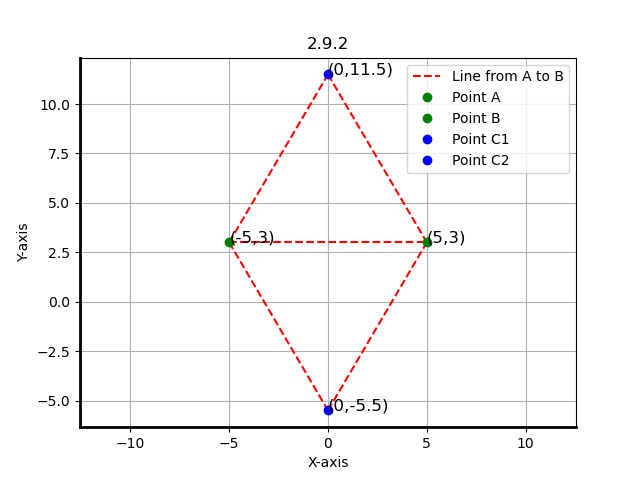
\includegraphics[width=0.8\columnwidth]{figs/fig1.png}
    \caption{2D Plot}
    \label{3D Plot}
\end{figure}

\end{document}
